\documentclass[11]{article}
\usepackage{lgrind}
\usepackage{fullpage}
\usepackage{graphicx}
\usepackage{xtab}

\author{Bo Shi}
\title{6.111 Lab Report 2 \\ Traffic Light Controller}
\date{October 13, 2004}


\begin{document}

\maketitle

\begin{abstract}
This report details the design and implementation of a relatively simple
traffic light controller.  The intersection for which this controller is being
designed also has a walk lamp and traffic sensor (along one street).  A
high--level overview of the design is followed by a detailed low--level
description on a module--by--module basis.  This report concludes with the
testing and debugging procedure used in the development of the traffic
controller.
\end{abstract}

\newpage
% \pagenumbering{roman}
% \setcounter{page}{1}
\tableofcontents

\newpage
\listoffigures 
\listoftables 

\newpage
% \pagenumbering{arabic}
% \setcounter{page}{1}
\section{Design Overview}
	\subsection{Requirements}
	This documents details the design for a traffic light controller at the
	intersection of Main Street and Side Street.  Both street lights are
	capable of sending a red, yellow, and green signal.  A walk signal is also
	available for pedestrians.  When the walk signal is on, all vehicle is
	halted.  A sensor is installed on Side street to monitor traffic.  The
	timing for each set of light signals depends on two things --- the values
	programmed into the controller by user input, and traffic conditions on
	Side Street.  If Side street has heavy traffic, Main Street's green signal
	length is shortened.  Conversely, Side street's green signal is lengthened
	under heavy traffic conditions.

	\subsection{Setup}
	The traffic light controller accepts four asynchronous inputs and two
	2-bit and 4-bit synchronized inputs and has a seven bit output
	controlling the switching of the traffic lights and the walk signal.
	The four asynchronous inputs to the controller are push buttons serving
	the following roles:
	\begin{itemize}
		\item Resetting the traffic light controller
		\item Sensor data from the streets
		\item Walk requests from pedestrians\footnote{It is assumed that all corners of the intersection have a walk request and that all requests will be sent as a single signal using a wired--OR.}
		\item Reprogram request
	\end{itemize}

	The two synchronized inputs allow control over the duration which
	various states last (for example, one may change the duration of
	yellow-light intervals).  The output is a 7-bit value ordered as
	Table~\ref{tbl:output} shows.  The FPGA used is an Altera Flex 10K10
	clocked with a 1.8432 Mhz crystal oscillator.
	\begin{table}
	\topcaption{Output Setup}
	\centering
		\begin{tabular}{|c|c|c|c|c|c|c|}
		\hline
		Bit 6 & Bit 5 & Bit 4 & Bit 3 & Bit 2 & Bit 1 & Bit 0 \\ \hline
		Main Red & Main Yellow & Main Green & Side Red & Side Yellow & Side Green & Walk \\ \hline
		\end{tabular}
	\label{tbl:output}
	\end{table}
	

	\subsection{Module Overview}
		\subsubsection{Synchronizer}
		This module synchronizes asynchronous input from the
		push buttons.  The RESET, WALK\_REQUEST, and REPROGRAM
		signals are converted to pulses while the SENSOR input
		is only synchronized.

		\subsubsection{Walk Register}
		The walk register is a very simple module containing a
		register and some additional control logic.  A walk
		request pulse will set the value in the register high
		and the signal will remain high until after the request
		as been granted.

		\subsubsection{Finite State Machine (FSM)}
		The specifications for operation are discussed in
		subsequent sections.  The FSM determines the output of the
		traffic light controller at any given time based on
		timing information retrieved from the time modules.

		\subsubsection{Time Parameters}
		This module determines the duration of a given state
		as requested by the FSM module.  Three different
		durations are available (see Figure 

		\subsubsection{Timer}
		At the request of the FSM, the timer module begins counting down a
		duration specified by the Time Parameters module and signals the
		FSM upon the end of the time duration.

		\subsubsection{Divider}
		The divider sends out a pulse every second.

\section{Module Implementation}
	\begin{figure}[h]
	\centering
	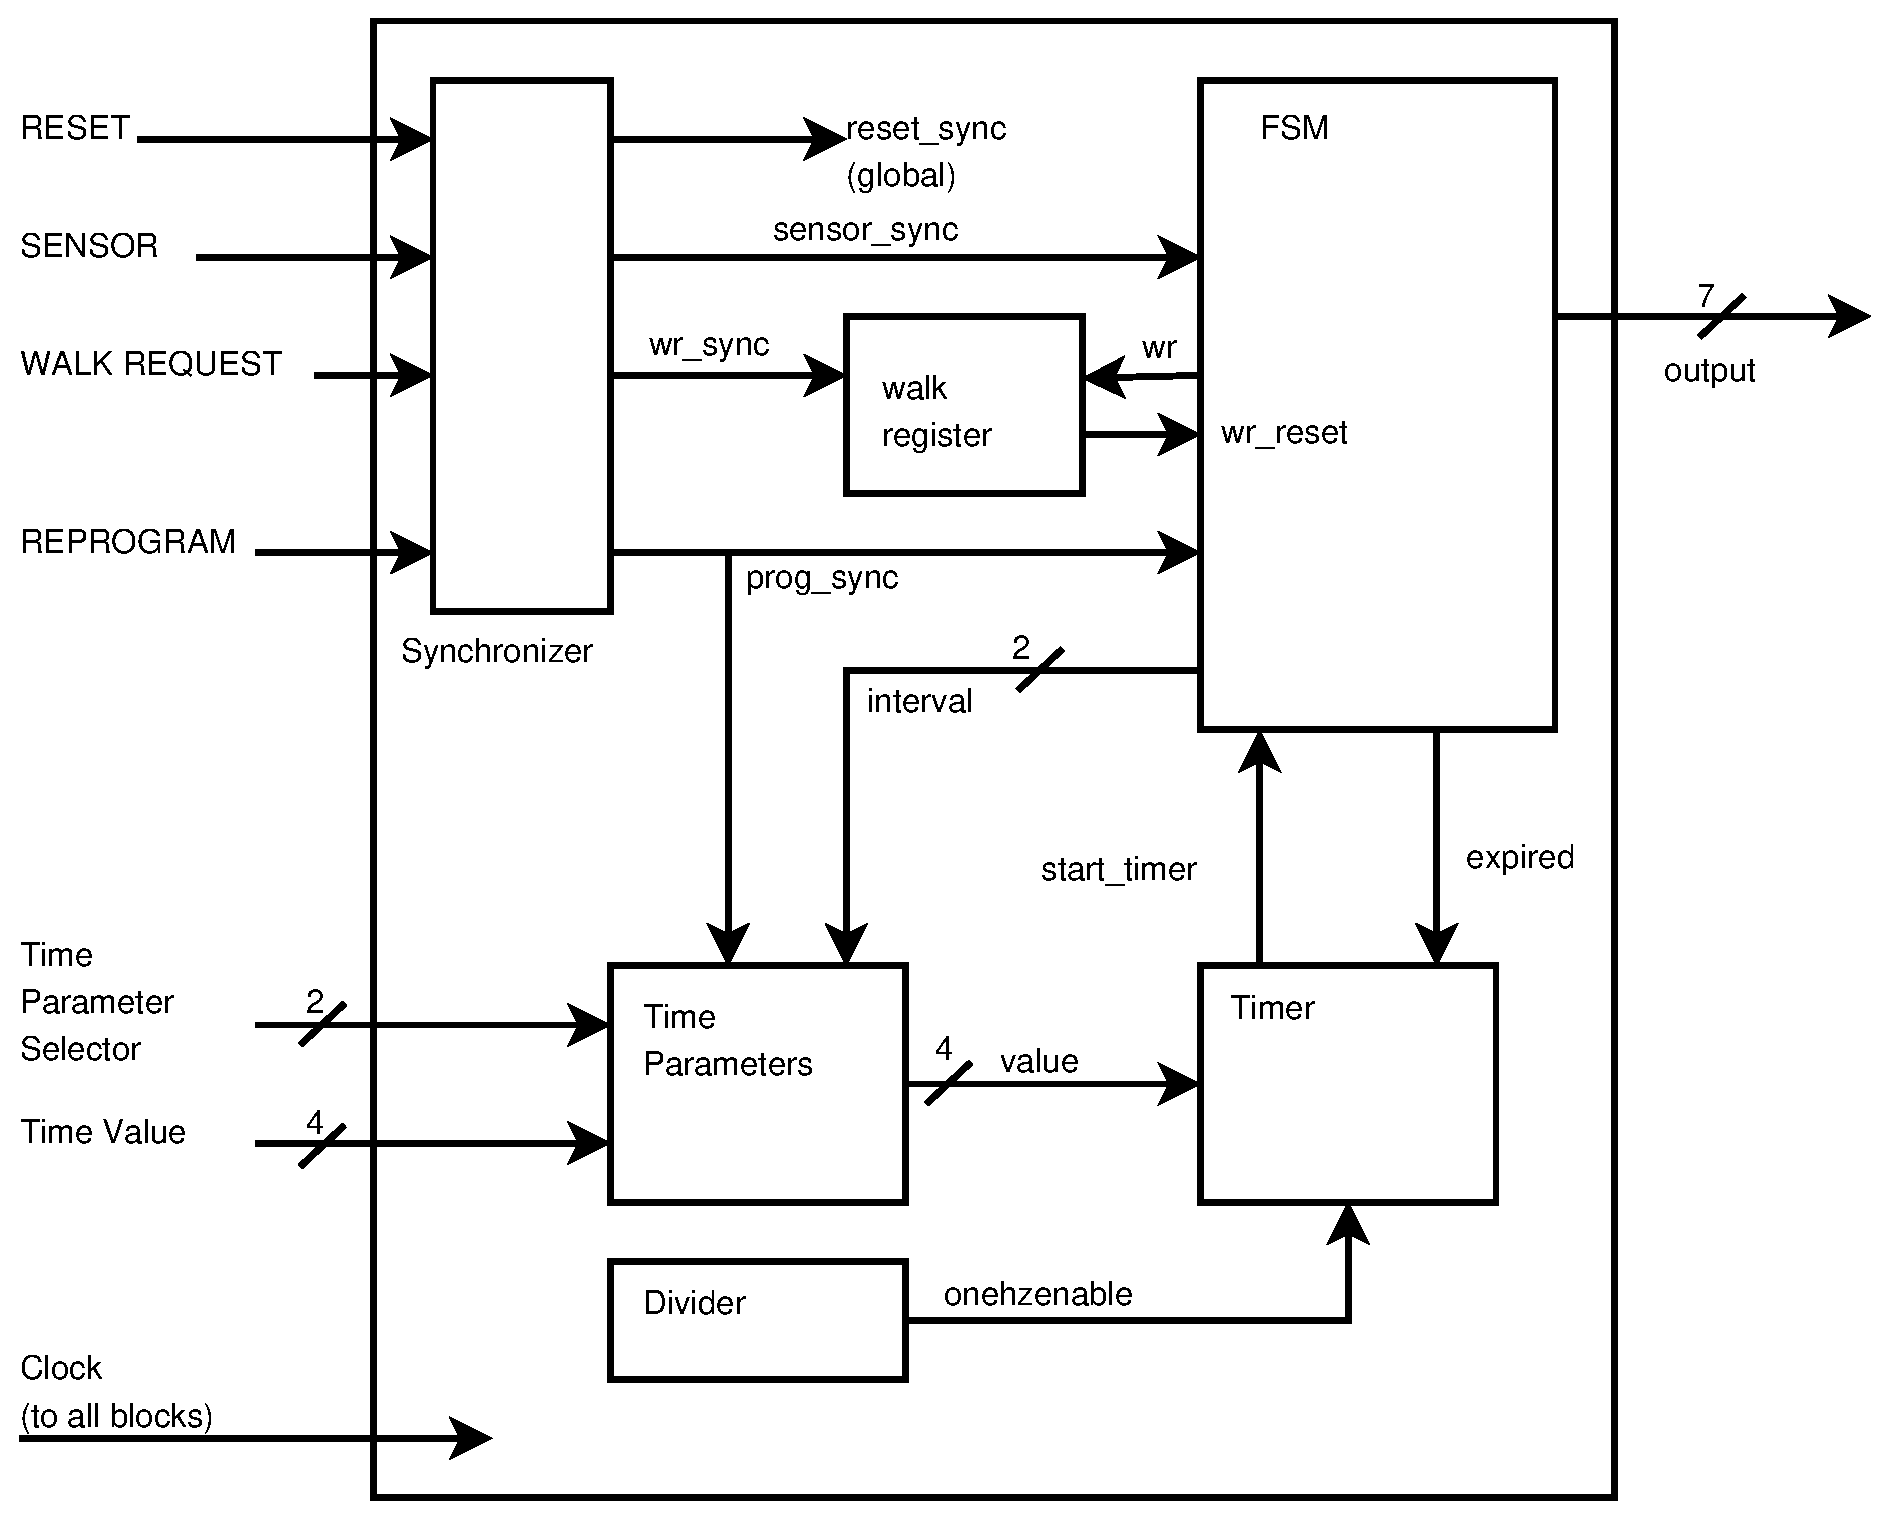
\includegraphics[scale=0.4]{block.ps}
	\caption{Block diagram of the modules inside the traffic light controller.}
	\label{fig:block}
	\end{figure}
	\subsection{Walk Register}
	The walk register module has an internal bit that is set to high when a
	walk signal, \texttt{wr\_sync}, has been requested.  The \texttt{wr}
	output of the walk register module is held high until this request is
	honored.  When the FSM exits the \texttt{S\_walk} state, a
	\texttt{wr\_reset} pulse is sent by the FSM and the register is set to
	a value of zero.

	\subsection{Timer}
	The timer keeps an internal 4-bit counter.  When it receives a
	\texttt{onehzenable} pulse from the Divider module, the counter decrements.
	When the counter's value is one, it sends out an {\texttt{expired}}
	pulse to the FSM.  Upon reception of a \texttt{start\_timer}
	pulse, the Timer will load a new counter value (the \texttt{value}
	signal) from the Time Parameter module and begin counting down.  The
	timer module is notified whenever 1 second elapses by a
	\texttt{onehzenable} pulse from the Divider module.

	\subsection{Time Parameters}
	This module maintains a table of integer values which represent
	the correct duration of a given state.  The data that this module
	provides is used by the Timer module to count the duration of the FSM's
	current state so that it can notify the FSM to change state.  The timer
	module provides timing data according to the state of the FSM (through
	the 2-bit \texttt{interval} signal).  The default timing values are
	given in Table~\ref{tbl:timeparam}.

	The specification also states that the time parameters should be
	programmable.  On the \texttt{prog\_sync} pulse, the module will read
	the 4--bit time value (the input ``Time Value'' in
	Figure~\ref{fig:block} and program the interval selected by the 2--bit
	select signal\footnote{It is assumed that these signals are in steady
	state when the reprogram button is pushed so that a synchronizer is not
	necessary.} (the input ``Time Parameter Selector'').  It is possible
	that an error might cause a value of zero might be programmed as one of
	the time parameters.  Since the \texttt{expired} signal is only sent
	when the timer counter has value 1, a programmed value of zero will
	simply cause the time parameter to become 16 seconds long because the
	value in the register will simply wrap around to 0xF when 1 is
	subtracted from 0.

	\subsection{Divider}
	The divider maintains a N--bit counter capable of holding a
	value larger and or equal to the clock frequency. Twenty--one bits was the
	minimum.  The clock used for the traffic light controller is a 1.8432 Mhz
	crystal oscillator.  Consequently, each time the Divider counter reached
	1,843,200, the counter is reset and the \texttt{onehzenable} pulse is sent
	to the Timer.

	\begin{figure}
	\centering
	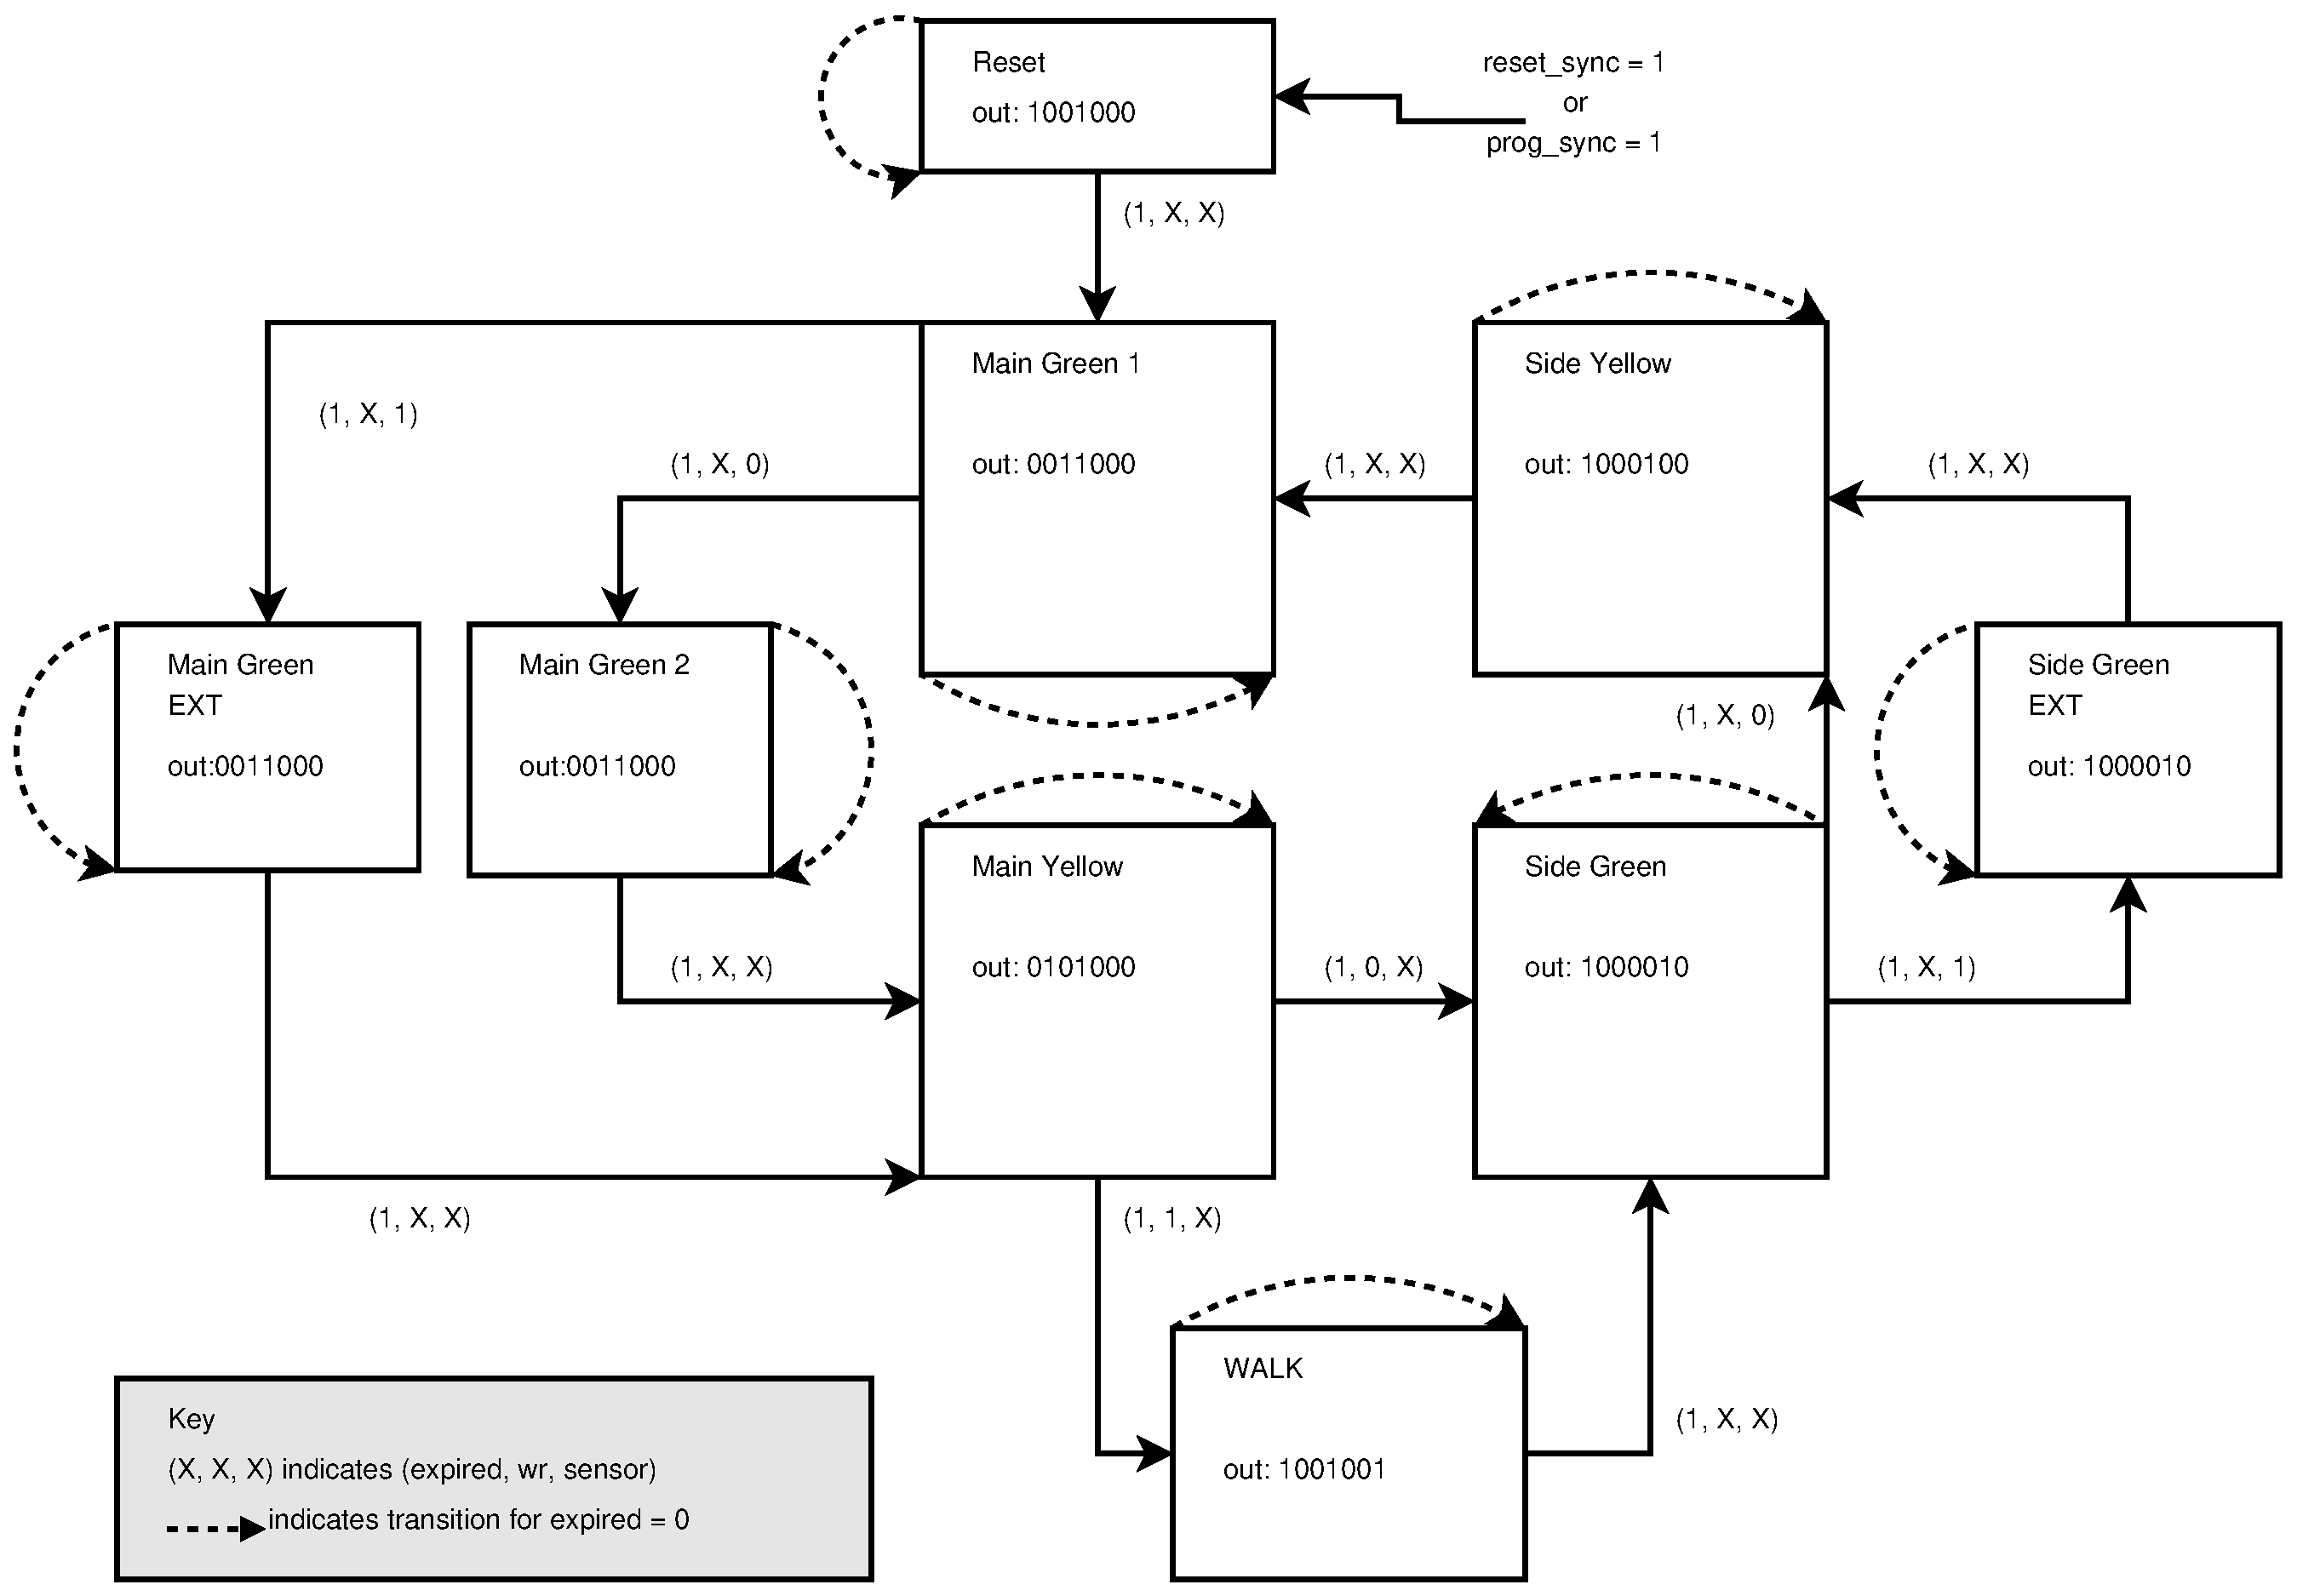
\includegraphics[scale=0.33]{fsm.ps}
	\caption{Finite State Machine for the Traffic Light Controller}
	\label{fig:fsm}
	\end{figure}

	\subsection{Finite State Machine}
	When RESET is asserted, the FSM enters the \texttt{S\_RESET}
	state\footnote{The original design used \texttt{S\_main\_green} as both
	the initial state and the reset state.  This was changed because the
	behavior of the design is not particularly safe.  If the reset were to
	be asserted during actual operation, it would be best to have a period
	of all red lights so that actual traffic does not get adversely
	confused.}.  The \texttt{S\_RESET} state lasts for 3 seconds and then
	the controller starts normal operation.  As indicated by the state
	transition diagram (Figure~\ref{fig:fsm}), the default duration of Main Street's
	green light is $2 \cdot t_{base}$.  For Side Street, green signals will
	only last $t_{base}$ seconds. The default duration of any Yellow signal
	is $t_{ext}$.  The controller will behave normally unless the sensor
	detects traffic or a walk signal has been requested (\texttt{sensor} or
	\texttt{wr} signal is high).  In these cases, the new states will go
	according to what the state transition diagram shows;  a walk interval
	will occur \emph{only} after a Main Street yellow signal and the green signal
	will lengthen for Side Street or shorten for Main Street if the sensor
	detects traffic on Side Street.

	The \texttt{RESET} state is entered when the reset button is pushed or
	when the program button is pushed.
	When a \texttt{prog\_sync} pulse is sent, the Timer Parameters module
	reprograms itself and so the FSM should enter into the \texttt{RESET}
	state.  This type of transition into the \texttt{RESET} state may occur
	from any state.
	
	\begin{table}
	\topcaption{Default Timing Parameters}
	\centering
		\begin{tabular}{|c|c|c|c|c|}
		\hline
		Interval Name & Symbol & Parameter Number & Default $\Delta$t (s) & Time Value \\ \hline
		Base & $t_{base}$ & \texttt{00} & 6 & \texttt{0110} \\ \hline
		Extended & $t_{ext}$ & \texttt{01} & 3 & \texttt{0011} \\ \hline
		Yellow & $t_{yel}$ & \texttt{10} & 2 & \texttt{0010} \\ \hline
		\end{tabular}
	\label{tbl:timeparam}
	\end{table}


\section{Testing and Debugging}
	The testing process is a repetitive cycle of simulation, wiring/burning
	FPGA's, and functional testing.  It is a good idea to test that all the
	pins of the FPGA and all the interconnects are working before debugging, as
	a lot of time was wasted attempting to solve problems caused by bad pins.

	\subsection{Module--by--Module Simulation}
	To simulate the system practically, the divider had to be altered so
	that each ``second'' lasted only a short number of clock cycles.  Ten
	was arbitrarily chosen as the number of clock cycles per divider pulse.
	The first step in testing was to test each module individually to make
	sure that they behaved correctly.  During this phase of testing, only
	the timer module seemed not to have the correct output.
	
	The problem was that the \texttt{expired} pulse was being sent out one
	second late.  This was due to an off--by--one error in the Verilog code
	which sent the pulse when the internal counter reached zero.  This was
	fixed by having the pulse sent out whenever the counter reached one.
	Luckily, this also resolved the secondary issue of how to handle programmed
	time intervals of zero.  Before this fix, attempting to program 0 into the
	time parameters would cause the FSM to lock into the \texttt{S\_RESET}
	state.  A careful eye toward timing was lacking and a subtle problem was
	missed.  This will be discussed next.

	\subsection{Wiring and Functional Testing}
	After all the modules had been tested individually, they were linked
	together in a top--level module and the finished code was burned onto
	the Altera Flex 10k10 chip.  At first, the controller seemed to be
	working correctly, but timing tests quickly revealed that the Time Parameter
	module seemed to be working incorrectly, as the duration for each state
	was off.  At this point, I went back into the simulator and simulated
	the whole controller.  A check of the simulation results revealed that
	the Timer was grabbing the value to count one clock cycle too early.

	The most complex interaction was between the FSM, Time Parameter, and
	Timer module.  The MUX was synchronized -- this caused a problem where
	the initial test results reported that there was an off-by-one error
	for the intervals.  The Timer was receiving `value' signals one clock
	cycle too early.  The method used to fix this was to use an additional
	register in the Timer module to delay the reading of value given by the
	Time Parameter module.  Further simulation ran correctly.  Another possible
	method which may have solved this problem was to hard-wire the mux using
	combinational logic (put select and value output outside of the
	\emph{always} block and use \texttt{assign} statements).  Aside from wiring
	and lab--kit issues, there were no further problems from this point on.


\section{Conclusions}
	After everything seemed to be working, a TA pointed out that I had
	misunderstood one of the requirements.  If the sensor was tripped
	while Main Street was green, my time duration for the green light would
	have been $2 \cdot t_{base} + t_{ext}$.  Fortunately, it was a simple
	matter to fix this.  Next time, I would write out the requirements in list
	form and in the testing phase, check them off each time a test was
	completed.  More accounting of this sort would have reduced the number of
	times that the FPGA was burned and this more organized and systematic
	method would most likely save time.

	Another lesson learned was that having all modules simulate correctly does
	not ensure that integration will go smoothly.  For the labs so far, I have
	dedicated the majority of my time to simulation, but I was careless
	integrating all the modules together.  In the future, more care should
	be given to the timing requirements of the modules.

\newpage
\section{Appendix A: Simulation Waveforms}
	The following are a listing of simulation waveforms for the Finite State
	Machine, the Synchronization module, and the Walk Register module.

	\begin{figure}[h]
	\centering
	\includegraphics[scale=0.40]{sim1.ps}
	\caption{Waveform of FSM under normal operation.  Note that the \texttt{expired} pulse is artificially generated.}
	\label{fig:sim1}
	\end{figure}

	\begin{figure}[h]
	\centering
	\includegraphics[scale=0.40]{sim2.ps}
	\caption{FSM with sensor operation.}
	\label{fig:sim2}
	\end{figure}

	\begin{figure}[h]
	\centering
	\includegraphics[scale=0.40]{sim3.ps}
	\caption{FSM with walk request then \texttt{prog\_sync} pulse.  Note how a reprogram request also resets the FSM.}
	\label{fig:sim3}
	\end{figure}

	\begin{figure}[h]
	\centering
	\includegraphics[scale=0.40]{sim4.ps}
	\caption{FSM with walk request then \texttt{reset} pulse.}
	\label{fig:sim4}
	\end{figure}

	\begin{figure}[h]
	\centering
	\includegraphics[scale=0.40]{sim6.ps}
	\caption{Synchronizer simulation waveform.  All asynchronous inputs are changed to pulses except for the sensor signal.}
	\label{fig:sim6}
	\end{figure}

	\begin{figure}[h]
	\centering
	\includegraphics[scale=0.40]{sim7.ps}
	\caption{Walk Register operation.}
	\label{fig:sim7}
	\end{figure}

\clearpage

\newpage
\section{Appendix B: Source Code Listing}
	\subsection{Step to Pulse Module}
	\begin{lgrind}
	\input exsync.v.latex
	\end{lgrind}

	\subsection{Synchronizer}
	\begin{lgrind}
	\input synchronizer.v.latex
	\end{lgrind}

\subsection{Walk Register}
	\begin{lgrind}
	\input walkregister.v.latex
	\end{lgrind}

\subsection{Finite State Machine}
	\begin{lgrind}
	\input fsm.v.latex
	\end{lgrind}

\subsection{Time Parameters}
	\begin{lgrind}
	\input timeparams.v.latex
	\end{lgrind}

\subsection{Timer}
	\begin{lgrind}
	\input timer.v.latex
	\end{lgrind}

\subsection{Divider}
	\begin{lgrind}
	\input divider.v.latex
	\end{lgrind}

\subsection{Top Level Module}
	\begin{lgrind}
	\input controller.v.latex
	\end{lgrind}

\end{document}
